% Define important features for the document
\documentclass[12pt,oneside]{article}
\setlength{\parindent}{0pt}
\setlength{\parskip}{4pt}

% Import packages
\usepackage[margin = 1in]{geometry}
\usepackage{amsfonts, amsmath, amssymb, amsthm, calc, centernot, color, csquotes, dsfont, enumitem, environ, fancyhdr, fontawesome5, graphicx, hyperref, marvosym, mathrsfs, mathtools, tcolorbox, titlesec}
\usepackage[flushmargin,hang]{footmisc}
\tcbuselibrary{breakable}

% Define toggles
\newif\ifsolutions
\solutionstrue % Toggle for instructor version
% \solutionsfalse % Toggle for student version

% Define size and spacing of section and subsection
\titleformat{\section}
  {\normalfont\large\bfseries}
  {\thesection}{1em}{}
\titleformat{\subsection}
  {\normalfont\normalsize\bfseries}
  {\thesubsection}{1em}{}
\titlespacing*{\section}{0pt}{6pt}{6pt} % ({left}{before}{after})
\titlespacing*{\subsection}{0pt}{6pt}{6pt} % ({left}{before}{after})

% Define commands
\newcommand{\indep}{\perp\!\!\!\perp}
\newcommand{\notindep}{\mathrel{\not\!\perp\!\!\!\perp}}
\newcommand{\E}{\mathbb{E}}
\newcommand{\Var}{\text{Var}}
\newcommand{\Cov}{\text{Cov}}
\newcommand{\Corr}{\text{Corr}}
\newcommand{\SD}{\text{SD}}
\newcommand{\SE}{\text{SE}}
\newcommand{\Bias}{\text{Bias}}
\newcommand{\MSE}{\text{MSE}}
\newcommand{\Risk}{\text{Risk}}
\newcommand{\Like}{\mathcal{L}}
\newcommand{\boot}{\text{boot}}
\newcommand{\strat}{\text{strat}}
\newcommand{\supp}{\text{supp}}
\newcommand{\MLE}{\text{MLE}}
\newcommand{\MoM}{\text{MoM}}
\newcommand{\MOM}{\text{MOM}}
\newcommand{\OLS}{\text{OLS}}
\newcommand{\LS}{\text{LS}}
\newcommand{\MAP}{\text{MAP}}
\newcommand{\MAE}{\text{MAE}}
\newcommand{\LP}{\text{LP}}
\newcommand{\HT}{\text{HT}}
\newcommand{\JS}{\text{JS}}
\newcommand{\RB}{\text{RB}}
\newcommand{\UB}{\text{UB}}
\newcommand{\DIM}{\text{DIM}}
\newcommand{\PATE}{\text{PATE}}
\newcommand{\SATE}{\text{SATE}}
\newcommand{\VIF}{\text{VIF}}
\newcommand{\GVIF}{\text{GVIF}}
\newcommand{\AIC}{\text{AIC}}
\newcommand{\BIC}{\text{BIC}}
\newcommand{\LASSO}{\text{LASSO}}
\newcommand{\PSS}{\text{PSS}}
\newcommand{\CV}{\text{CV}}
\newcommand{\logit}{\text{logit}}
\newcommand{\odds}{\text{odds}}
\newcommand{\OR}{\text{OR}}
\newcommand{\N}{\mathcal{N}}
\newcommand{\Bern}{\text{Bern}}
\newcommand{\Bin}{\text{Bin}}
\newcommand{\Beta}{\text{Beta}}
\newcommand{\Gam}{\text{Gamma}}
\newcommand{\Expo}{\text{Expo}}
\newcommand{\Pois}{\text{Pois}}
\newcommand{\Unif}{\text{Unif}}
\newcommand{\DUnif}{\text{DUnif}}
\newcommand{\Geom}{\text{Geom}}
\newcommand{\FS}{\text{FS}}
\newcommand{\NBin}{\text{NBin}}
\newcommand{\HGeom}{\text{HGeom}}
\newcommand{\Mult}{\text{Mult}}
\newcommand{\MVN}{\text{MVN}}
\newcommand{\IG}{\text{IG}}
\newcommand{\Tweedie}{\text{Tweedie}}
\newcommand{\simiid}{\overset{\text{i.i.d.}}{\sim}}
\newcommand{\simind}{\overset{\text{ind.}}{\sim}}
\newcommand{\simnull}{\overset{H_0}{\sim}}
\newcommand{\simapprox}{\overset{\cdot}{\sim}}
\newcommand{\R}{\mathbb{R}}
\newcommand{\Z}{\mathbb{Z}}
\newcommand{\Q}{\mathbb{Q}}
\newcommand{\C}{\mathbb{C}}
\newcommand{\I}{\mathbb{I}}
\newcommand{\indic}{\mathds{1}}
\newcommand{\iid}{\text{i.i.d.}}
\newcommand{\Ind}{\text{Ind}}
\newcommand{\SSq}{\text{SSq}}
\newcommand{\trace}{\text{trace}}
\newcommand{\rank}{\text{rank}}
\newcommand{\diag}{\text{diag}}
\newcommand{\adj}{\text{adj}}
\newcommand{\SSE}{\text{SSE}}
\newcommand{\SST}{\text{SST}}
\newcommand{\SSR}{\text{SSR}}
\newcommand{\GLS}{\text{GLS}}
\newcommand{\ti}{\text{time}}
\newcommand{\outcome}{\text{outcome}}
\newcommand{\exposure}{\text{exposure}}
\newcommand{\NA}{\text{NA}}
\newcommand{\cp}{\text{cp}}
\newcommand{\tip}{\textbf{\faLightbulb}: }
\newcommand{\warning}{\textbf{\Biohazard}: }
\newcommand{\blank}[1][4cm]{\underline{\hspace{#1}}}

% Define theorem-style environment (italic body, bold header)
\newtheorem{theorem}{Theorem}
\newtheorem{lemma}{Lemma}
\newtheorem{proposition}{Proposition}
\newtheorem{corollary}{Corollary}

% Define definition-style environment (upright body, bold header)
\theoremstyle{definition}
\newtheorem{definition}{Definition}
\newtheorem{example}{Example}
\newtheorem{problem}{\faPen \ Problem}
\newtheorem{concept}{\faPen \ Concept Checker}
\newtheorem{challenge}{\faFire \ Challenge}
\newtheorem{activity}{\faDiceThree \ Activity}

% Define idea-style environment (unnumbered definition)
\newtheorem*{idea}{Idea}

% Define remark-style environment (upright body, italic header)
\theoremstyle{remark}
\newtheorem{remark}{Remark}

% Define environment for solution box
\newsavebox{\solutioncontentbox}
\NewEnviron{solutionbox}[1][Solution]{
  \sbox{\solutioncontentbox}{
    \begin{minipage}{\dimexpr\linewidth-2\fboxsep\relax}
      \BODY
    \end{minipage}
  }
  \ifsolutions
    \begin{tcolorbox}[
      title=#1,
      colback=gray!5,
      colframe=black,
      breakable
    ]
      \BODY
    \end{tcolorbox}
  \else
    \begin{tcolorbox}[
      title=#1,
      colback=white,
      colframe=black,
      breakable,
      height=\dimexpr\ht\solutioncontentbox+\dp\solutioncontentbox+1cm\relax
    ]
    \end{tcolorbox}
  \fi
}

% Begin document
\begin{document}
\pagestyle{fancy}
\fancyhead[L]{STAT 110: Introduction to Probability}
\fancyhead[R]{Fall 2026}
\begin{center}
\bf \Large
Section 4: Expectation and Variance \\[0.5em]
\normalsize
Avery Kim (\href{mailto:averykim@college.harvard.edu}{\texttt{averykim@college.harvard.edu}}), \\[0.2em]
Ricky Truong (\href{mailto:rickytruong@college.harvard.edu}{\texttt{rickytruong@college.harvard.edu}})
\end{center}

% Section: Introduction
\section{Introduction}

\subsection{Logistics}

Welcome! The goal of our weekly section is to review content from lecture, with emphasis on big-picture intuition, mathematical derivation, and hands-on practice.

Specifically, we aim for section to be interactive, well-paced, inclusive, and fun! Please do not hesitate to reach out if you have any questions/feedback!

\subsection{Office Hours}

$\bullet$ See the Google Calendar for the most accurate information!

\subsection{Attendance}

$\bullet$ \href{https://bit.ly/stat110harvard}{\texttt{bit.ly/stat110harvard}}

% Section: Expectation
\section{Expectation}

\begin{idea}
Often, we describe a random variable with its \textit{expectation}, which captures the center of its distribution. Even though most random variables can crystallize to a wide range of values, the expectation is a useful statistic to describe the center or long-run average of the distribution.
\end{idea}

\subsection{Fundamentals}

\begin{definition}[Expectation]
For a random variable $X$, $\E[X]$ is its \textit{expectation}.

$\bullet$ Informally, $\E[X]$ is the \textit{weighted average} of $X$, where we weigh each possible \textit{crystallization} by its associated probability.

$\bullet$ Mathematically, \[\E[X] = \sum_{x \in \supp(X)} \underbrace{x}_{\text{value}} \underbrace{P(X = x)}_{\text{PMF at value}}.\]

$\bullet$ E.g., let $X \sim \Bern(\frac{1}{3})$, with support $\{0, 1\}$. Thus, \[P(X = 0) = \frac{2}{3}, \ P(X = 1) = \frac{1}{3},\] so \[\E[X] = \sum_{x \in \{0, 1\}} x P(X = x) = \left( 0 \times \frac{2}{3} \right) + \left( 1 \times \frac{1}{3} \right) = \frac{1}{3}.\]
\end{definition}

\begin{concept}
Let $X$ be the value from rolling a fair 6-sided die. Find $\E[X]$.
\end{concept}

\begin{solutionbox}
$\E[X] = 1(\frac{1}{6}) + 2(\frac{1}{6}) + 3(\frac{1}{6}) + 4(\frac{1}{6}) + 5(\frac{1}{6}) + 6(\frac{1}{6}) = 3.5$.
\end{solutionbox}

\begin{concept}
Why is $\E[X]$ a valid expression but $P(X)$ is not?
\end{concept}

\begin{solutionbox}
$X$ is a random variable, not an event! Expectation takes a random variable as input and returns a number as output. Probability takes an event as input and returns a number (between $0$ and $1$) as output.
\end{solutionbox}

\subsection{Expectation Toolkit}

\begin{definition}[Linearity of expectation]
For random variables $X$ and $Y$ and constants $a$, $b$, and $c$, \[\E[aX + bY + c] = a \E[X] + b \E[Y] + c.\]

$\bullet$ We call $c$ a \textit{degenerate} random variable, where it crystallizes to $c$ with probability $1$.
\end{definition}

\begin{definition}[Fundamental bridge]
The expectation of an \textit{indicator} for an event $A$ is $P(A)$—i.e., \[\E[\indic\{A\}] = P(A).\]
\end{definition}

\begin{proof}
Let $X \sim \Bern(p)$. Thus, $X = 0$ with probability $1 - p$ and $X = 1$ with probability $p$. By definition of expectation, $\E[X] = 0 (1 - p) + 1 (p) = p$, so the expectation of a Bernoulli random variable is $p$. If $\indic\{A\}$ is an indicator for an event $A$, then $\indic\{A\} \sim \Bern(P(A))$.
\end{proof}

\begin{definition}[Law of the Unconscious Statistician (LOTUS)]
For a random variable $X$ and function $g: \R \rightarrow \R$, \[\E[g(X)] = \sum_{x \in \supp(X)} g(x) P(X = x).\]

$\bullet$ Notice that we still use the PMF of $X$ to find $\E[g(X)]$!
\end{definition}

\begin{concept}
If we want to find $\E[X^2]$ using LOTUS, what is $g(X)$ and $g(x)$?
\end{concept}

\begin{solutionbox}
$g$ is the function applied to $X$ within the expectation. Thus, $g(X) = X^2$—the function applied to the random variable—and $g(x) = x^2$—the function applied to an arbitrary crystallized value.
\end{solutionbox}

% Section: Variance
\section{Variance}

\begin{idea}
In addition to expectation, \textit{variance} is used to describe a random variable—specifically, its spread/uncertainty.
\end{idea}

\subsection{Fundamentals}

\begin{definition}[Variance]
For a random variable $X$, $\Var[X]$ is its \textit{variance}.

$\bullet$ Informally, $\Var[X]$ is a measure of the \textit{spread} of $X$—i.e., how far does $X$ tend to be from its expectation?

$\bullet$ Mathematically, \[\Var[X] = \E[(X - \E[X])^2] = \E[X^2] - (\E[X])^2.\]

$\bullet$ \tip Often, it's easier to use $\Var[X] = \E[X^2] - (\E[X])^2$ and LOTUS to find $\E[X^2]$.
\end{definition}

\begin{definition}[Standard deviation]
For a random variable $X$, $\SD[X]$ is its \textit{standard deviation}.

$\bullet$ Mathematically, \[\SD[X] = \sqrt{\Var[X]}.\]
\end{definition}

\begin{concept}
By definition, variance is the expected squared deviation of a random variable from its expectation—i.e., $\Var[X] = \E[(X - \E[X])^2]$. Show that $\Var[X] = \E[X^2] - (\E[X])^2$.
\end{concept}

\begin{solutionbox}
First, let $\mu = \E[X]$ to make the notation cleaner. Notice that $\mu$ is just a constant (since expectation returns a number as output), so linearity of expectation applies.

\[
\begin{aligned}
\Var[X] &= \E[(X - \mu)^2] && \text{by definition} \\
&= \E[X^2 - 2X\mu + \mu^2] && \text{by FOIL} \\
&= \E[X^2] - 2\mu\E[X] + \mu^2 && \text{by linearity} \\
&= \E[X^2] - 2\mu^2 + \mu^2 && \text{since $\mu = \E[X]$} \\
&= \E[X^2] - \mu^2 && \text{by simplifying} \\
&= \E[X^2] - (\E[X])^2 && \text{since $\mu = \E[X]$}
\end{aligned}
\]
\end{solutionbox}

\subsection{Variance Toolkit}

\begin{center}
  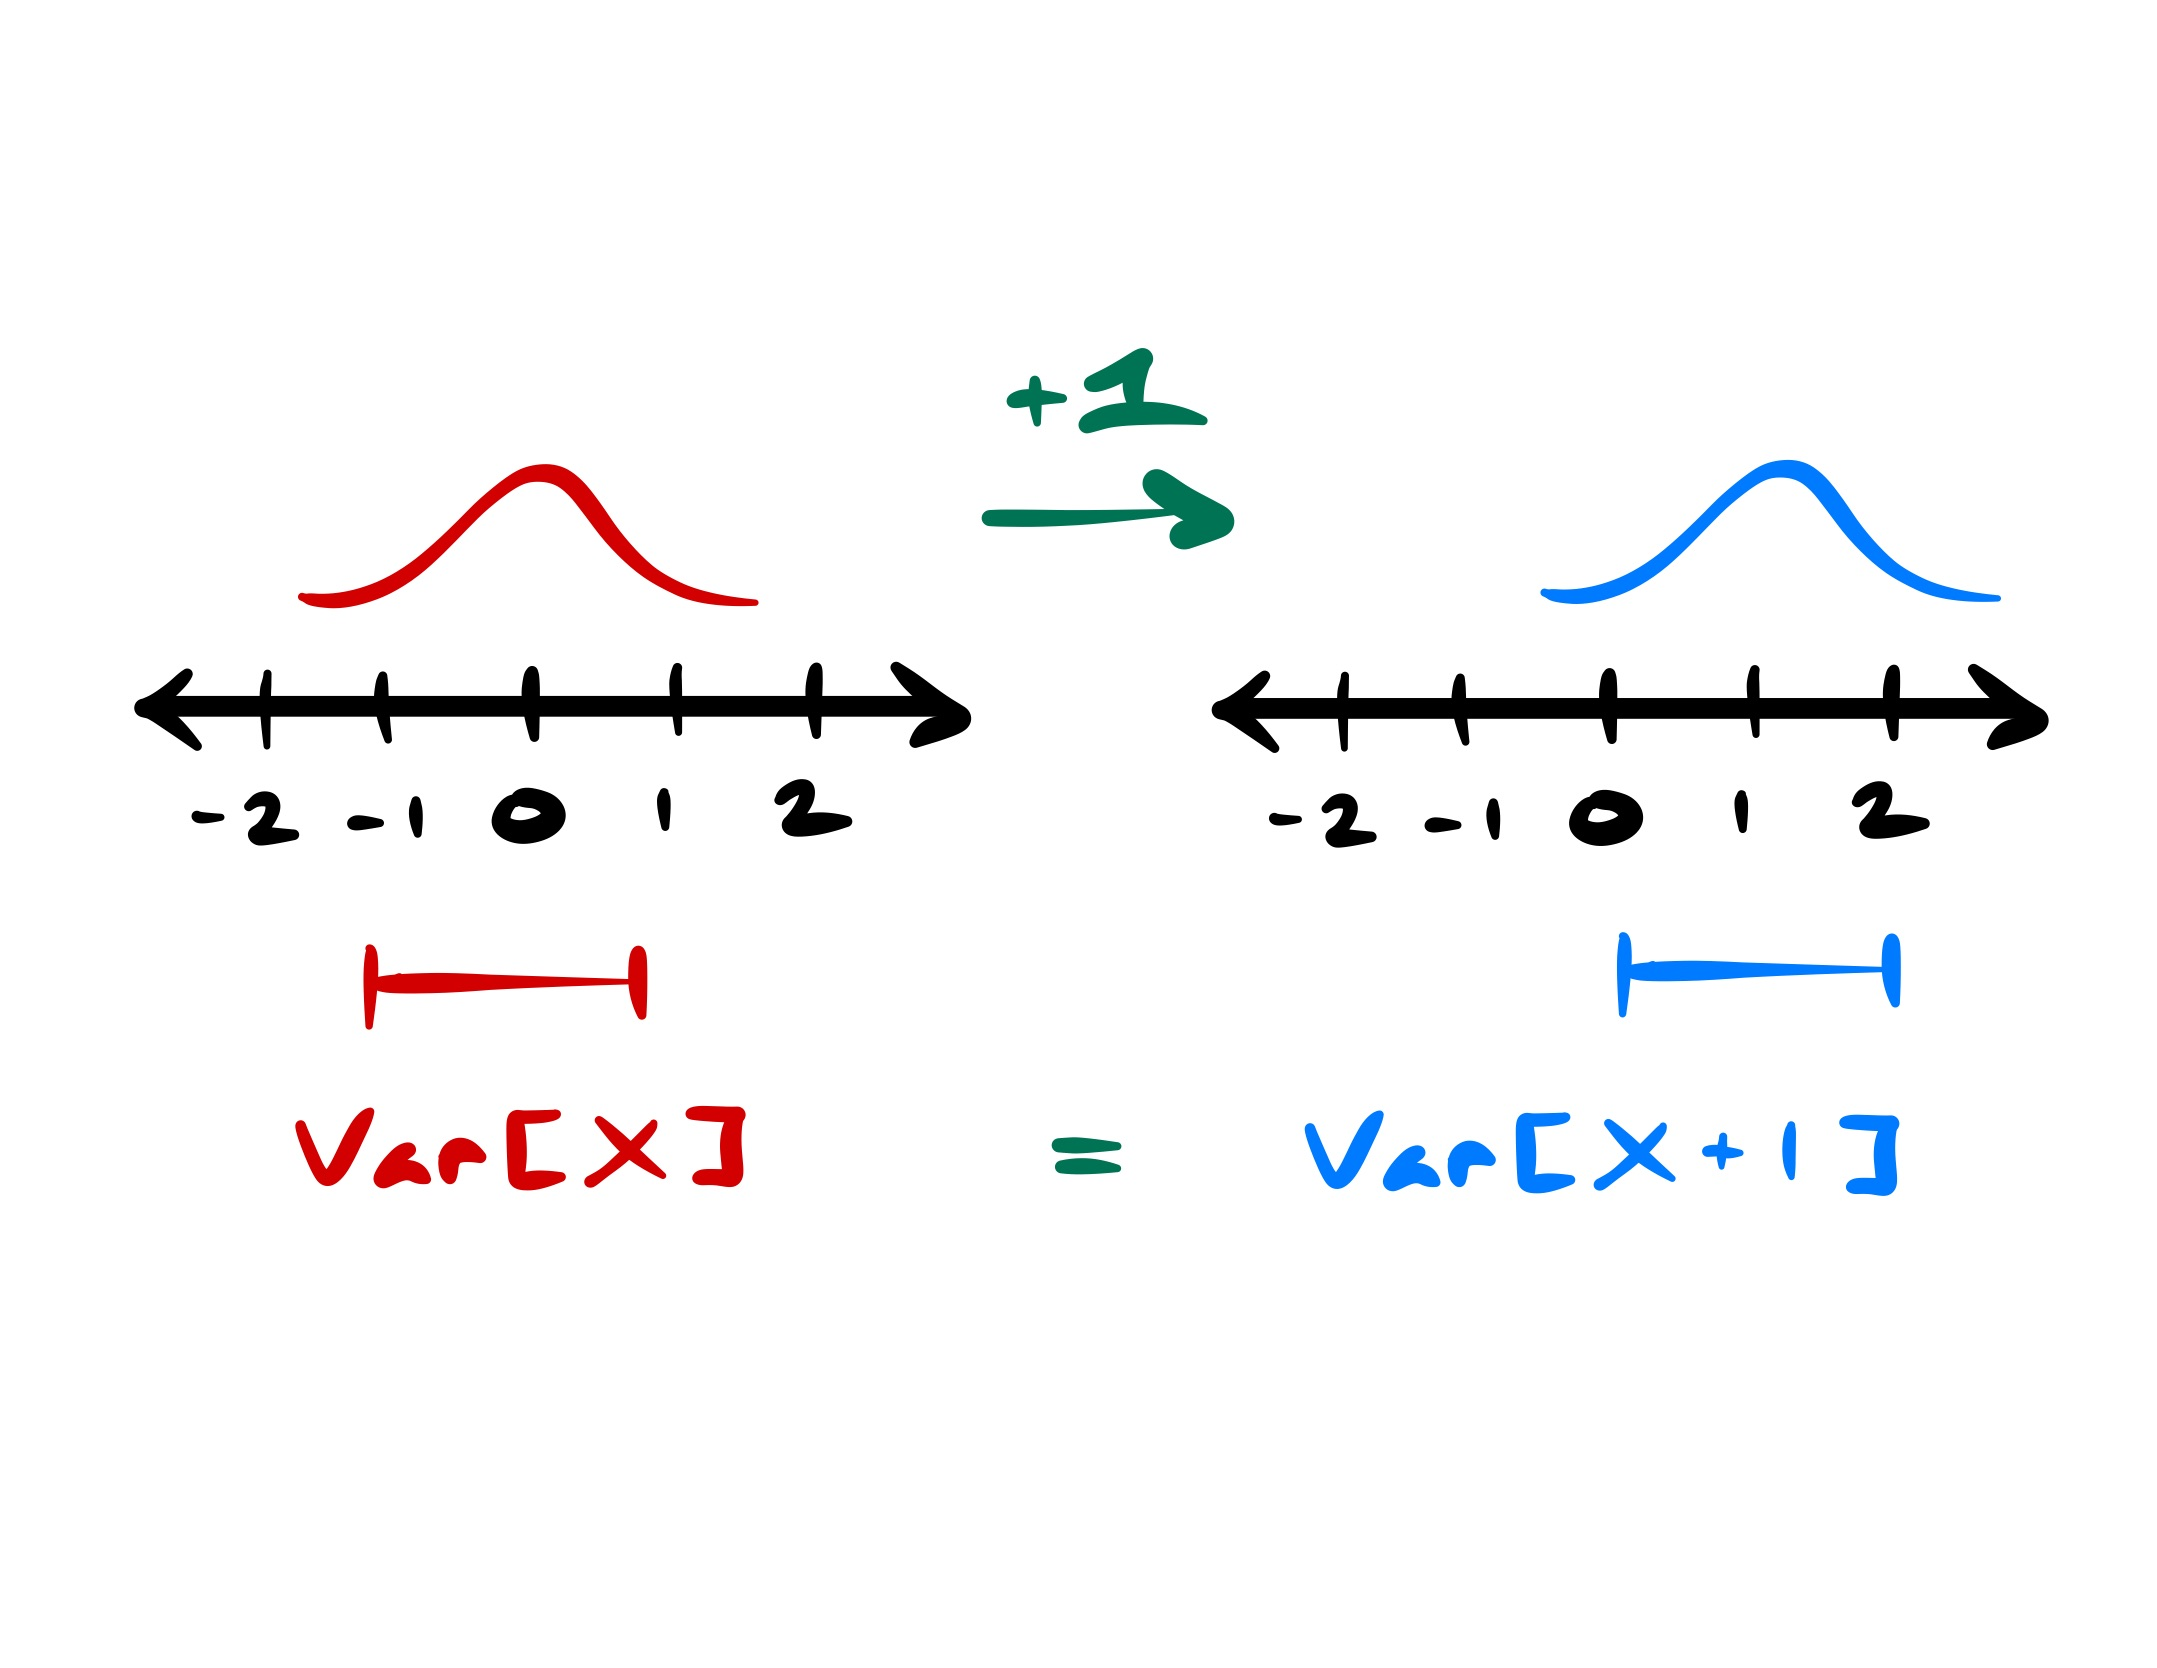
\includegraphics[width=0.5\textwidth]{stat110_section4_figure1.jpg}\\{\footnotesize FIGURE 1: Shifting by a constant does not change $\Var[X]$.}
\end{center}

\begin{definition}[Bilinearity of variance]
For a random variable $X$ and constants $a$ and $b$, \[\Var[aX + b] = a^2 \Var[X].\]
\end{definition}

\begin{definition}[Sum of independent random variables]
If $X_1, \ldots, X_n$ are independent, then \[\Var[X_1 + \ldots + X_n] = \Var[X_1] + \ldots + \Var[X_n].\]
\end{definition}

\begin{definition}[Nonnegativity of variance]
For a random variable $X$, \[\Var[X] \geq 0.\]
\end{definition}

% Section: Expectation and Variance of Famous Distributions
\section{Expectation and Variance of Famous Distributions}

\begin{idea}
The \textit{famous distributions} we've previously mentioned have known expectations and variances, which makes our lives easier! 
\end{idea}

\begin{example}[Bernoulli]
Let $X$ be distributed \textit{Bernoulli} with parameter $p$—i.e., \[X \sim \Bern(p).\] Then \[\E[X] = p, \ \Var[X] = p (1 - p).\]
\end{example}

\begin{concept}
Let $X \sim \Bern(p)$, with support $\{0, 1\}$. We showed that $\E[X] = p$.\footnote{See Definition 3.} Show that $\Var[X] = p (1 - p)$.
\end{concept}

\begin{solutionbox}
$\Var[X] = \E[X^2] - (\E[X])^2$. First, $\E[X] = p$, so $(\E[X])^2 = p^2$. Next, $\E[X^2] = \sum_{x \in \supp(X)} x^2 P(X = x)$ by LOTUS. We can simplify this to $\E[X^2] = 0^2 (1 - p) + 1^2 p = p$, so $\Var[X] = \E[X^2] - (\E[X])^2 = p - p^2 = p (1 - p)$. For some intuition, $X$ can only crystallize to $0$ or $1$, and $0^2 = 0$ while $1^2 = 1$.
\end{solutionbox}

\begin{example}[Binomial]
Let $X$ be distributed \textit{Binomial} with parameters $n$ and $p$—i.e., \[X \sim \Bin(n, p).\] Then \[\E[X] = np, \ \Var[X] = n p (1 - p).\]
\end{example}

\begin{concept}
Let $X \sim \Bin(n, p)$. Show that $\E[X] = n p$ and $\Var[X] = n p (1 - p)$.
\end{concept}

\begin{solutionbox}
By the story/property of the Binomial, $X = Y_1 + \ldots + Y_n$, where $Y_1, \ldots, Y_n \simiid \Bern(p)$.

\[
\begin{aligned}
\E[X] &= \E[Y_1 + \ldots + Y_n] && \text{by substituting} \\
&= \E[Y_1] + \ldots + \E[Y_n] && \text{by linearity} \\
&= p + \ldots + p && \text{by expectation of Bernoulli} \\
&= n p && \text{by simplifying }
\end{aligned}
\]

\[
\begin{aligned}
\Var[X] &= \Var[Y_1 + \ldots + Y_n] && \text{by substituting} \\
&= \Var[Y_1] + \ldots + \Var[Y_n] && \text{by sum of independent random variables} \\
&= p (1 - p) + \ldots + p (1 - p) && \text{by variance of Bernoulli} \\
&= n p (1 - p) && \text{by simplifying }
\end{aligned}
\]
\end{solutionbox}

\begin{example}[Geometric]
Let $X$ be distributed \textit{Geometric} with parameter $p$—i.e., \[X \sim \Geom(p).\] Then \[\E[X] = \frac{1 - p}{p}, \ \Var[X] = \frac{1 - p}{p^2}.\]
\end{example}

\begin{concept}
Let $X \sim \FS(p)$. Find $\E[X]$ and $\Var[X]$.
\end{concept}

\begin{solutionbox}
By the story/property of First Success, $X = Y + 1$, where $Y \sim \Geom(p)$.

\[
\begin{aligned}
\E[X] &= \E[Y + 1] && \text{by substituting} \\
&= \E[Y] + 1 && \text{by linearity} \\
&= \frac{1 - p}{p} + 1 && \text{by expectation of Geometric} \\
&= \frac{1}{p} && \text{by simplifying }
\end{aligned}
\]

\[
\begin{aligned}
\Var[X] &= \Var[Y + 1] && \text{by substituting} \\
&= \Var[Y] && \text{by bilinearity} \\
&= \frac{1 - p}{p^2} && \text{by variance of Geometric}
\end{aligned}
\]
\end{solutionbox}

\begin{example}[Negative Binomial]
Let $X$ be distributed \textit{Negative Binomial} with parameters $r$ and $p$—i.e., \[X \sim \NBin(r, p).\] Then \[\E[X] = r \left( \frac{1 - p}{p} \right), \Var[X] = r \left( \frac{1 - p}{p^2} \right).\]
\end{example}

\begin{example}[Hypergeometric]
Let $X$ be distributed \textit{Hypergeometric} with parameters $w$, $b$, and $n$—i.e., \[X \sim \HGeom(w, b, n).\] Then \[\E[X] = \frac{nw}{b + w}, \ \Var[X] = \left( \frac{nwb}{(w + b)^2} \right) \left( \frac{w + b - n}{w + b - 1} \right).\]
\end{example}

% Section: Poisson Distribution
\section{Poisson Distribution}

\begin{idea}
The final discrete distribution we'll introduce is the \textit{Poisson} distribution, which is unique in that its story is a bit complicated. However, many real-world phenomena are modeled using the Poisson as an \textit{approximation}.
\end{idea}

\subsection{Fundamentals}

\begin{definition}[Poisson]
Let $X$ be distributed \textit{Poisson} with parameter $\lambda$—i.e., \[X \sim \Pois(\lambda).\]

$\bullet$ \textbf{Story}: $X$ is the number of occurrences for a rare event with rate $\lambda$ in $t$ units of time/space (with $t = 1$ as default).

$\bullet$ \textbf{Example}: Let $X$ be the number of calls received in an hour at a customer service desk, which receives an average of 4 calls per hour. Then $X \sim \Pois(4)$.

$\bullet$ \textbf{PMF and Support}: \[P(X = x) = \frac{e^{- \lambda} \lambda^x}{x!}\] for $x \in \{0, 1, \ldots\}$.

$\bullet$ \textbf{Properties}: If $X \sim \Pois(\lambda_1)$ and $Y \sim \Pois(\lambda_2)$ with $X \indep Y$, then \[X + Y \sim \Pois(\lambda_1 + \lambda_2)\] and \[X \mid \{X + Y = n\} \sim \Bin \left( n, \frac{\lambda_1}{\lambda_1 + \lambda_2} \right).\]
\end{definition}

\begin{concept}
If $X$ is the number of calls received in an hour and $X \sim \Pois(4)$, then what is the distribution of the number of calls received in \textit{two} hours?
\end{concept}

\begin{solutionbox}
Let $Y$ be the number of calls received in two hours. $Y \sim \Pois(8)$ since the rate is $4$ calls in $1$ unit of time, and we're now concerned with $t = 2$.
\end{solutionbox}

\begin{definition}[Connection between Poisson and Binomial]
If $X \sim \Bin(n, p)$ and we let $n \rightarrow \infty$ and $p \rightarrow 0$ such that $\lambda = np$ remains fixed, then the PMF of $X$ converges to the PMF of $\Pois(\lambda)$.
\end{definition}

\begin{definition}[Poisson paradigm]
Let $A_1, \ldots, A_n$ be independent (or weakly dependent) events, where $p_i = P(A_i)$. If $X = \sum_{i = 1}^{n} \indic\{A_i\}$ is the number of events that occur (with $n$ large and $p_i$ small), then $X$ is \textit{approximately} distributed $\Pois(\lambda)$, where $\lambda = \sum_{i = 1}^{n} p_i$.

$\bullet$ We denote this \textit{approximate distribution} as $X \simapprox \Pois(\lambda)$.
\end{definition}

\begin{definition}[Chicken-egg story]
Suppose that a chicken lays $N$ eggs, where $N \sim \Pois(\lambda)$. Each egg independently hatches with probability $p$ and fails to hatch with probability $q = 1 - p$. Let $X$ be the number of eggs that hatch and $Y$ be the number of eggs that don't hatch (such that $X + Y = N$). The \textit{joint PMF} of $X$ and $Y$, $P(X = x, Y = y)$, is the product of two terms, where one relies only on $x$ and the other relies only on $y$—i.e., \[P(X = x, Y = y) = \left( \frac{e^{- \lambda p} (\lambda p)^x}{x!} \right) \left( \frac{e^{- \lambda q} (\lambda q)^y}{y!} \right) = P(X = x) P(Y = y).\]

$\bullet$ Mathematically, if $N \sim \Pois(\lambda)$ and $X \mid \{N = n\} \sim \Bin(n, p)$, then \[X \sim \Pois(\lambda p)\] and \[Y = N - X \sim \Pois(\lambda q),\] with \[X \indep Y.\]

$\bullet$ \tip Often, we apply the chicken-egg story when $N \sim \Pois(\lambda)$ is split into 2 groups: successes (with probability $p$) and failures (with probability $q = 1 - p$).
\end{definition}

\begin{concept}
In a certain election, there are $V \sim \Pois(\lambda)$ registered voters. Each registered voter is a Democrat with probability $p$ and a Republican with probability $1 - p$, independent of other voters. Each registered voter actually votes in the election with probability $s$ and stays home with probability $1 - s$, independent of other voters and independent of party affiliations. Let $X$ be the number of registered Democrats who actually vote in the election. What is the distribution of $X$?\footnote{Inspired by Problem 2 in \enquote{Practice Midterm 2} by Joseph K. Blitzstein.}
\end{concept}

\begin{solutionbox}
$X \sim \Pois(\lambda p s)$ by chicken-egg story. Notice that we're \enquote{splitting} the Poisson random variable $V$.
\end{solutionbox}

\subsection{Expectation and Variance of Poisson}

\begin{example}[Poisson]
Let $X$ be distributed \textit{Poisson} with parameter $\lambda$—i.e., \[X \sim \Pois(\lambda).\] Then \[\E[X] = \lambda, \ \Var[X] = \lambda.\]
\end{example}

% Section: Table of Distributions
\section{Table of Distributions}

\begin{idea}
We conclude with a review of the famous distributions we've covered so far.
\end{idea}

\begin{center}
{
\tiny
\renewcommand{\arraystretch}{1.5}
\begin{tabular}{p{2cm}|p{2.5cm}|p{3cm}|p{1.5cm}|p{2.5cm}|p{2.5cm}}
\textbf{Name} & \textbf{Story} & \textbf{PMF \& Support} & \textbf{Expectation} & \textbf{Variance} & \textbf{Properties} \\ \hline

$X \sim \Bern(p)$
& $X$ succeeds (i.e., $X = 1$) with probability $p$ and fails (i.e., $X = 0$) with probability $1 - p$
& $P(X = x) = p^x (1 - p)^{1 - x}$ for $x \in \{0, 1\}$
& $p$
& $p (1 - p)$ \\

\hline

$X \sim \Bin(n, p)$
& $X$ is the number of successes in $n$ independent trials that each have success probability $p$
& $P(X = x) = \binom{n}{x} p^x (1 - p)^{n - x}$ for $x \in \{0, 1, \ldots, n\}$
& $n p$
& $n p (1 - p)$
& If $X \sim \Bin(n, p)$ and $Y \sim \Bin(m, p)$ with $X \indep Y$, then $X + Y \sim \Bin(n + m, p)$; If $X_1, \ldots, X_n \simiid \Bern(p)$, then $X_1 + \ldots + X_n \sim \Bin(n, p)$ \\

\hline

$X \sim \Geom(p)$
& $X$ is the number of failures until we observe a success in independent trials that each have success probability $p$, \textit{not} counting that first success
& $P(X = x) = (1 - p)^{x} p$ for $x \in \{0, 1, \ldots\}$
& $\frac{1 - p}{p}$
& $\frac{1 - p}{p^2}$
& If $X \sim \Geom(p)$, then $X + 1 \sim \FS(p)$ \\

\hline

$X \sim \NBin(r, p)$
& $X$ is the number of failures until we observe the $r$th success in independent trials that each have success probability $p$, \textit{not} counting any successes
& $P(X = x) = \binom{x + r - 1}{r - 1} p^{r} (1 - p)^{x}$ for $x \in \{0, 1, \ldots\}$
& $r \left( \frac{1 - p}{p} \right)$
& $r \left( \frac{1 - p}{p^2} \right)$
& If $X_1, \ldots, X_r \simiid \Geom(p)$, then $X_1 + \ldots + X_r \sim \NBin(r, p)$ \\

\hline

$X \sim \HGeom(w, b, n)$
& $X$ is the number of \textit{desirable} objects in a sample if we draw $n$ objects, \textit{without replacement}, from a population with $w$ \textit{desirable} objects and $b$ \textit{undesirable} objects (with $w + b$ total objects)
& $P(X = x) = \frac{\binom{w}{x} \binom{b}{n - x}}{\binom{w + b}{n}}$ for $x \in \{\max(0, n - b), \ldots, \min(n, w)\}$
& $\frac{nw}{b + w}$
& $\left( \frac{nwb}{(w + b)^2} \right) \left( \frac{w + b - n}{w + b - 1} \right)$
& If $X \sim \Bin(n, p)$ and $Y \sim \Bin(m, p)$ with $X \indep Y$, then $X \mid \{X + Y = r\} \sim \HGeom(n, m, r)$ \\

\hline

$X \sim \Pois(\lambda)$
& $X$ is the number of occurrences for a rare event with rate $\lambda$ in $t$ units of time/space (with $t = 1$ as default)
& $P(X = x) = \frac{e^{- \lambda} \lambda^x}{x!}$ for $x \in \{0, 1, \ldots\}$
& $\lambda$
& $\lambda$
& If $X \sim \Pois(\lambda_1)$ and $Y \sim \Pois(\lambda_2)$ with $X \indep Y$, then $X + Y \sim \Pois(\lambda_1 + \lambda_2)$ and $X \mid \{X + Y = n\} \sim \Bin \left( n, \frac{\lambda_1}{\lambda_1 + \lambda_2} \right)$
\end{tabular}
}
\end{center}

% Section: Exercises
\section{Exercises}

\begin{problem}
Suppose that Alice is taking a multiple choice exam that consists of $20$ questions. Each question has $5$ options but only $1$ correct answer. Unfortunately, Alice forgets to study and randomly guesses for each question.

(a) What is the probability that Alice answers all questions correctly?

(b) What is the expected number of questions Alice answers correctly?

(c) For this part only, suppose that the exam consists of \textit{checkbox} questions. Each question has $5$ options, and any number of them (from $0$ to $5$) may be correct. Alice answers each question by randomly choosing which options to check, and she answers the question correctly only if she checks all the correct options (and nothing more). A passing grade requires at least $75\%$ of the answers to be correct. What is the probability that Alice gets a passing grade? You may leave your answer as a sum.

(d) For this part only, suppose that the exam progresses in difficulty, with $i$ options for question $i \in \{1, \ldots, 20\}$ (e.g., question $4$ has $4$ options, question $5$ has $5$ options, and so on). Like before, each question has only $1$ correct answer. What is the expected number of questions Alice answers correctly? You may leave your answer as a sum.
\end{problem}

\begin{solutionbox}
(a) Let $Q_i$ be the event that Alice answers question $i$ correctly. By naive probability, $P(Q_i) = \frac{1}{5}$. Importantly, since Alice randomly guesses for each question, $Q_i \indep Q_j \ \forall \ i \neq j$. By the multiplication rule, $P(\text{Alice answers all questions correctly}) = \left( \frac{1}{5} \right)^{20}$, which is very small!

(b) Let $X$ be the number of questions Alice answers correctly. Notice that $X = \indic\{Q_{1}\} + \ldots + \indic\{Q_{20}\}$, and $\indic\{Q_{i}\} \simiid \Bern(\frac{1}{5})$. By the story of the Binomial, $X \sim \Bin(20, \frac{1}{5})$, so $\E[X] = (20)(\frac{1}{5}) = 4$.

(c) By the multiplication rule, for each question, there are $2^5 = 32$ possible subsets/ways to check the options (we can either check or not check each of the $5$ options), but only $1$ of those ways corresponds to the correct answer. By naive probability, $P(Q_i) = \frac{1}{32}$, so $X \sim \Bin(20, \frac{1}{32})$.

\[
\begin{aligned}
P(\text{Alice gets a passing grade}) &= P(X \geq 15) && \text{by definition of $X$} \\
&= \sum_{x = 15}^{20} P(X = x) && \text{since $X$ is discrete} \\
&= \sum_{x = 15}^{20} \binom{20}{x} \left( \frac{1}{32} \right)^x \left( \frac{31}{32} \right)^{20 - x} && \text{by Binomial PMF} \\
\end{aligned}
\]

(d) Importantly, $X$ is no longer Binomial since each question has a different success probability. By naive probability, $P(Q_i) = \frac{1}{i}$.

\[
\begin{aligned}
\E[X] &= \E \left[ \sum_{i = 1}^{20} \indic\{Q_i\} \right] && \text{since $X = \sum_{i = 1}^{20} \indic\{Q_i\}$} \\
&= \sum_{i = 1}^{20} \E[\indic\{Q_i\}] && \text{by linearity} \\
&= \sum_{i = 1}^{20} P(Q_i) && \text{by fundamental bridge} \\
&= \sum_{i = 1}^{20} \frac{1}{i} && \text{by naive probability} \\
&= 3.59773 && \text{by simplifying}
\end{aligned}
\]
\end{solutionbox}

\end{document}